\titlespacing*{\chapter}{0pt}{-1em}{2.6em}
\chapter[DONNÉES APRS DANS LES CHAMPS DESTINATION ET SOURCE AX.25]{Données APRS dans les champs Destination et Source
AX.25}\label{donnuxe9es-aprs-dans-les-champs-destination-et-source-ax.25}
\titlespacing*{\chapter}{0pt}{2.8em}{2.6em}

\begin{aprssideblock}{Le champ\\Destination Address\\AX.25}
\phantomsection\addcontentsline{toc}{section}{Le champ Destination Address AX.25}\label{le-champ-destination-address-ax.25}
Le champ Destination Address AX.25 peut contenir 6 types d'information APRS :

\begin{itemize}
\tightlist
\item
  Une adresse APRS générique.
\item
  Une adresse APRS générique avec un symbole.
\item
  Un numéro de version de logiciel APRS.
\item
  Des données encodées Mic-E.
\item
  Un Maidenhead Grid Locator (obsolète).
\item
  Une adresse Alternate Net (ALTNET).
\end{itemize}

Dans chacun de ces cas, le SSID de Destination Address peut spécifier un chemin
digipeater APRS générique.
\end{aprssideblock}

\begin{aprssideblock}{Adresses génériques\\de destination APRS}
\phantomsection\addcontentsline{toc}{section}{Adresses génériques de destination APRS}\label{adresses-guxe9nuxe9riques-de-destination-aprs}
APRS utilise les adresses génériques de type beacon suivantes :

\begin{center}
\ttfamily
\begin{tabular}{lllllll}
\lit{AIR}*† & \lit{CQ}* & \lit{DX}* & \lit{MAIL}* & \lit{RTCM}* & \lit{SYM}* & \lit{WX}* \\
\lit{ALL}* & \lit{DF}* & \lit{GPS}* & \lit{MICE}* & \lit{SKY}* & \lit{TEL}* & \lit{ZIP}*† \\
\lit{AP}* & \lit{DGPS}* & \lit{ID}* & \lit{QST}* & \lit{SPACE}* & \lit{TEST}* & \\
\lit{BEACON} & \lit{DRILL}* & \lit{JAVA}* & \lit{QTH}* & \lit{SPC}* & \lit{TLM}* & \\
\end{tabular}
\end{center}

L'astérisque est un joker permettant d'étendre l'adresse jusqu'à un total de
6 caractères alphanumériques. Ainsi, par exemple, \texttt{WX1}, \texttt{WX12}
et \texttt{WX12CD} sont toutes des adresses de destination APRS valides.

† Les adresses {\ttfamily \lit{AIR}*} et {\ttfamily \lit{ZIP}*} sont en cours
d'abandon, mais sont actuellement nécessaires pour assurer la compatibilité
avec les versions antérieures.

Toutes ces adresses ont un SSID de \texttt{-0}. Les SSID non nuls sont
réservés au digipeating APRS générique.

Ces adresses sont copiées par tous. Tous les logiciels APRS doivent accepter
les paquets comportant ces adresses de destination.

L'adresse \lit{GPS}, c'est-à-dire l'adresse exacte à 3 lettres \lit{GPS} et
non {\ttfamily \lit{GPS}*}, est spécifiquement destinée aux trackers qui
envoient des positions latitude/longitude par l'intermédiaire de digipeaters
capables de convertir les positions au format de données compressées.

Les adresses \lit{DGPS} et \lit{RTCM} sont utilisées par les stations de
correction GPS différentielle. La plupart des logiciels n'exploitent pas les
paquets utilisant ces adresses, si ce n'est pour les transmettre à un
récepteur GPS connecté.

L'adresse \lit{SKY} est utilisée par les stations Skywarn.

Les paquets adressés à {\ttfamily \lit{SPC}L} sont destinés aux événements
spéciaux. Les logiciels APRS peuvent afficher ces paquets à l'exclusion de
tous les autres, afin de réduire à l'écran l'encombrement produit par les
autres stations ne participant pas à l'événement spécial.

Les adresses \lit{TEL} et \lit{TLM} sont utilisées par les stations de
télémétrie.
\end{aprssideblock}

\begin{aprssideblock}{Adresse générique\\avec symbole}
\phantomsection\addcontentsline{toc}{section}{Adresse générique avec symbole}\label{adresse-guxe9nuxe9rique-avec-symbole}
APRS utilise plusieurs des adresses génériques énumérées ci-dessus d'une
manière particulière, afin de spécifier non seulement une adresse, mais aussi
un symbole d'affichage. Ces adresses particulières sont
{\ttfamily \lit{GPS}xyz}, {\ttfamily \lit{GPS}Cnn},
{\ttfamily \lit{GPS}Enn}, {\ttfamily \lit{SPC}xyz} et
{\ttfamily \lit{SYM}xyz}. Elles sont destinées aux cas dans lesquels il est
impossible d'inclure le symbole dans le champ Information AX.25.

Les adresses {\ttfamily \lit{GPS}…} ci-dessus sont destinées à un usage
général.

Les adresses {\ttfamily \lit{SPC}…} sont destinées aux événements spéciaux.

Les adresses {\ttfamily \lit{SYM}…} sont réservées à un usage futur.

Les caractères \texttt{xy} et \texttt{nn} désignent des entrées des tables de
symboles APRS. Le caractère \texttt{z} spécifie un overlay de symbole. Voir le
chapitre 20 : Symboles APRS et l'annexe 2 pour plus d'informations.
\end{aprssideblock}

\begin{aprssideblock}{Numéro de version\\du logiciel APRS}
\phantomsection\addcontentsline{toc}{section}{Numéro de version du logiciel APRS}\label{numuxe9ro-de-version-de-logiciel-aprs}
Le champ Destination Address AX.25 peut contenir le numéro de version du
logiciel APRS exécuté par la station. La connaissance du numéro de version
peut être utile lors du débogage.

Les types de versions logicielles suivants sont réservés (\texttt{xx} et
\texttt{xxx} indiquent un numéro de version) :

\begin{center}
\begin{tabular}{@{}ll@{}}
{\ttfamily \lit{APC}xxx} & APRS/CE, Windows CE \\
{\ttfamily \lit{APD}xxx} & Linux aprsd server \\
{\ttfamily \lit{APE}xxx} & PIC-Encoder \\
{\ttfamily \lit{API}xxx} & Icom radios (futur) \\
{\ttfamily \lit{APIC}xx} & ICQ messaging \\
{\ttfamily \lit{APK}xxx} & Kenwood radios \\
{\ttfamily \lit{APM}xxx} & MacAPRS \\
{\ttfamily \lit{APP}xxx} & pocketAPRS \\
{\ttfamily \lit{APR}xxx} & APRSdos \\
\lit{APRS} & anciennes versions d'APRSdos \\
{\ttfamily \lit{APRS}M} & anciennes versions de MacAPRS \\
{\ttfamily \lit{APRS}W} & anciennes versions de WinAPRS \\
{\ttfamily \lit{APS}xxx} & APRS+SA \\
{\ttfamily \lit{APW}xxx} & WinAPRS \\
{\ttfamily \lit{APX}xxx} & X-APRS \\
{\ttfamily \lit{APY}xxx} & Yaesu radios (futur) \\
{\ttfamily \lit{APZ}xxx} & Expérimental \\
\end{tabular}
\end{center}

Cette table sera complétée par l'APRS Working Group.
Par exemple, une station utilisant la version 3.2.6 de MacAPRS pourrait
utiliser l'indicatif de destination {\ttfamily \lit{APM}326}.
La destination expérimentale est réservée à un usage temporaire seulement
pendant le développement d'un produit, avant qu'une adresse spéciale APRS
Software Version lui soit attribuée.
\end{aprssideblock}

\begin{aprssideblock}{Données Mic-E\\encodées}
\phantomsection\addcontentsline{toc}{section}{Données Mic-E encodées}\label{donnuxe9es-mic-e-encoduxe9es}
Une autre utilisation possible du champ Destination Address AX.25 consiste à
y placer des données encodées Mic-E. Ces données comprennent :

\begin{itemize}
\tightlist
\item
  La latitude de la station.
\item
  Un indicateur West/East et un indicateur Longitude Offset, utilisés dans les
  calculs de longitude.
\item
  Un Message Code.
\item
  Le chemin digipeater APRS.
\end{itemize}

Ces données sont utilisées avec les données associées dans le champ
Information AX.25 pour fournir un Position Report complet et d'autres
informations sur la station (voir chapitre 10 : Format de données Mic-E).
\end{aprssideblock}

\begin{aprssideblock}{Maidenhead Grid\\Locator dans\\Destination Address}
\phantomsection\addcontentsline{toc}{section}{Maidenhead Grid Locator dans Destination Address}\label{maidenhead-grid-locator-en-destination}
Le champ Destination Address AX.25 peut contenir un Maidenhead Grid Locator à
6 caractères. Par exemple : \texttt{IO91SX}. Ce format est généralement
utilisé par les opérateurs meteor scatter et satellite qui doivent conserver
des paquets aussi courts que possible.
Ce format est maintenant obsolète.
\end{aprssideblock}

\begin{aprssideblock}{Alternate Nets}
\phantomsection\addcontentsline{toc}{section}{Alternate Nets}\label{alternate-nets}
Toute autre adresse de destination ne figurant pas dans la liste
générique spécifique ni dans les autres catégories mentionnées ci-dessus
peut être utilisée dans des Alternate Nets (ALTNETs) par des groupes
d'individus à des fins spéciales. Ils peuvent ainsi utiliser
l'infrastructure APRS pour une variété d'expérimentations sans encombrer
les cartes et les listes des autres stations APRS. Seules les stations
utilisant la même adresse ALTNET devraient voir leurs données.
\end{aprssideblock}

\begin{aprssideblock}{Chemin digipeater\\APRS générique}
\phantomsection\addcontentsline{toc}{section}{Chemin digipeater APRS générique}\label{chemin-digipeater-aprs-guxe9nuxe9rique}
Le SSID dans le champ Destination Address de tous les paquets est encodé
pour spécifier le chemin digipeater APRS.

Si le SSID de Destination Address est \texttt{-0}, le paquet suit le
chemin digipeater AX.25 standard (« VIA ») contenu dans le champ
Digipeater Addresses de la trame AX.25.

Si le SSID de Destination Address est non nul, le paquet suit l'un des 15
chemins digipeater APRS génériques.

\clearpage
Le champ SSID dans la Destination Address, c'est-à-dire dans le 7e octet
d'adresse, est encodé comme suit :

{\sffamily\bfseries Chemins digipeater APRS dans le SSID de Destination Address}

\begin{flushleft}
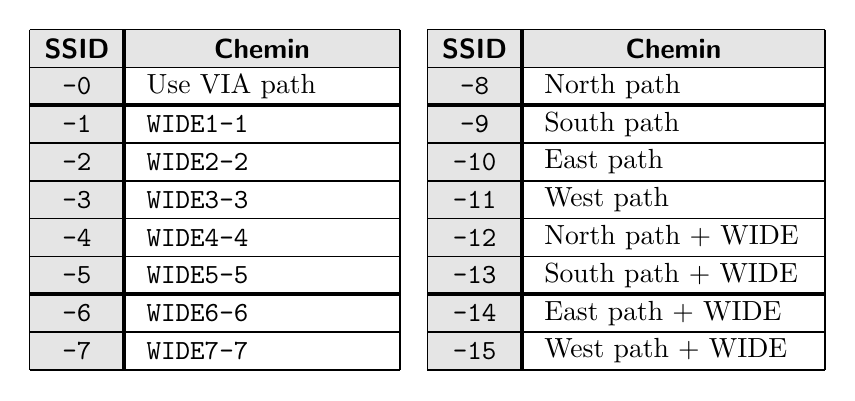
\begin{tikzpicture}[x=1cm,y=1cm,baseline=(current bounding box.north)]
  \def\rowheight{0.48}
  \def\ssidwidth{1.20}

  \begin{scope}
    \def\tablewidth{4.70}
    \fill[gray!20] (0,0) rectangle (\tablewidth,-\rowheight);
    \fill[gray!20] (0,-\rowheight) rectangle (\ssidwidth,{-9*\rowheight});
    \foreach \line in {0,...,9}
      \draw[line width=0.5pt] (0,{-\line*\rowheight}) -- (\tablewidth,{-\line*\rowheight});
    \draw[line width=1.5pt] (0,{-2*\rowheight}) -- (\tablewidth,{-2*\rowheight});
    \draw[line width=1.5pt] (0,{-7*\rowheight}) -- (\tablewidth,{-7*\rowheight});
    \draw[line width=0.5pt] (0,0) -- (0,{-9*\rowheight});
    \draw[line width=1.5pt] (\ssidwidth,0) -- (\ssidwidth,{-9*\rowheight});
    \draw[line width=0.5pt] (\tablewidth,0) -- (\tablewidth,{-9*\rowheight});

    \node[font=\sffamily\bfseries] at ({\ssidwidth/2},{-0.5*\rowheight}) {SSID};
    \node[font=\sffamily\bfseries] at ({(\ssidwidth+\tablewidth)/2},{-0.5*\rowheight}) {Chemin};
    \foreach \ssid [count=\row from 1] in {0,1,2,3,4,5,6,7}
      \node[font=\ttfamily] at ({\ssidwidth/2},{-(\row+0.5)*\rowheight}) {-\ssid};
    \node[anchor=west] at ({\ssidwidth+0.16},{-1.5*\rowheight}) {Use VIA path};
    \foreach \wide [count=\row from 2] in {1,2,3,4,5,6,7}
      \node[anchor=west,font=\ttfamily] at ({\ssidwidth+0.16},{-(\row+0.5)*\rowheight}) {WIDE\wide-\wide};
  \end{scope}

  \begin{scope}[xshift=5.05cm]
    \def\tablewidth{5.05}
    \fill[gray!20] (0,0) rectangle (\tablewidth,-\rowheight);
    \fill[gray!20] (0,-\rowheight) rectangle (\ssidwidth,{-9*\rowheight});
    \foreach \line in {0,...,9}
      \draw[line width=0.5pt] (0,{-\line*\rowheight}) -- (\tablewidth,{-\line*\rowheight});
    \draw[line width=1.5pt] (0,{-2*\rowheight}) -- (\tablewidth,{-2*\rowheight});
    \draw[line width=1.5pt] (0,{-7*\rowheight}) -- (\tablewidth,{-7*\rowheight});
    \draw[line width=0.5pt] (0,0) -- (0,{-9*\rowheight});
    \draw[line width=1.5pt] (\ssidwidth,0) -- (\ssidwidth,{-9*\rowheight});
    \draw[line width=0.5pt] (\tablewidth,0) -- (\tablewidth,{-9*\rowheight});

    \node[font=\sffamily\bfseries] at ({\ssidwidth/2},{-0.5*\rowheight}) {SSID};
    \node[font=\sffamily\bfseries] at ({(\ssidwidth+\tablewidth)/2},{-0.5*\rowheight}) {Chemin};
    \foreach \ssid [count=\row from 1] in {8,9,10,11,12,13,14,15}
      \node[font=\ttfamily] at ({\ssidwidth/2},{-(\row+0.5)*\rowheight}) {-\ssid};
    \node[anchor=west] at ({\ssidwidth+0.16},{-1.5*\rowheight}) {North path};
    \node[anchor=west] at ({\ssidwidth+0.16},{-2.5*\rowheight}) {South path};
    \node[anchor=west] at ({\ssidwidth+0.16},{-3.5*\rowheight}) {East path};
    \node[anchor=west] at ({\ssidwidth+0.16},{-4.5*\rowheight}) {West path};
    \node[anchor=west] at ({\ssidwidth+0.16},{-5.5*\rowheight}) {North path + WIDE};
    \node[anchor=west] at ({\ssidwidth+0.16},{-6.5*\rowheight}) {South path + WIDE};
    \node[anchor=west] at ({\ssidwidth+0.16},{-7.5*\rowheight}) {East path + WIDE};
    \node[anchor=west] at ({\ssidwidth+0.16},{-8.5*\rowheight}) {West path + WIDE};
  \end{scope}
\end{tikzpicture}
\end{flushleft}
\end{aprssideblock}

\begin{aprssideblock}{SSID de Source\\Address\\pour spécifier\\les symboles}
\phantomsection\addcontentsline{toc}{section}{SSID de Source Address pour spécifier les symboles}\label{ssid-de-source-address-pour-spuxe9cifier-des-symboles}
Le champ Source Address AX.25 contient l'indicatif et le SSID de la station
d'origine. Si le SSID est \texttt{-0}, APRS ne le traite d'aucune manière
particulière.

Si, en revanche, le SSID de Source Address est non nul, APRS l'interprète
comme une icône d'affichage. Cette utilisation est exclusivement destinée aux
trackers autonomes pour lesquels il n'existe aucune autre méthode permettant
de spécifier un symbole d'affichage ou une adresse de destination, par exemple
les trackers MIM ou NMEA.

Pour plus d'informations, voir le chapitre 20 : Symboles APRS.
\end{aprssideblock}
